\begin{figure}[htbp]
	\centering

	 % \resizebox{12cm}{!}{\input{images/137SCTBayesianLinearRegressor.tikz}}


    \subfloat[AoR Bayesian linear regressor.]{
	  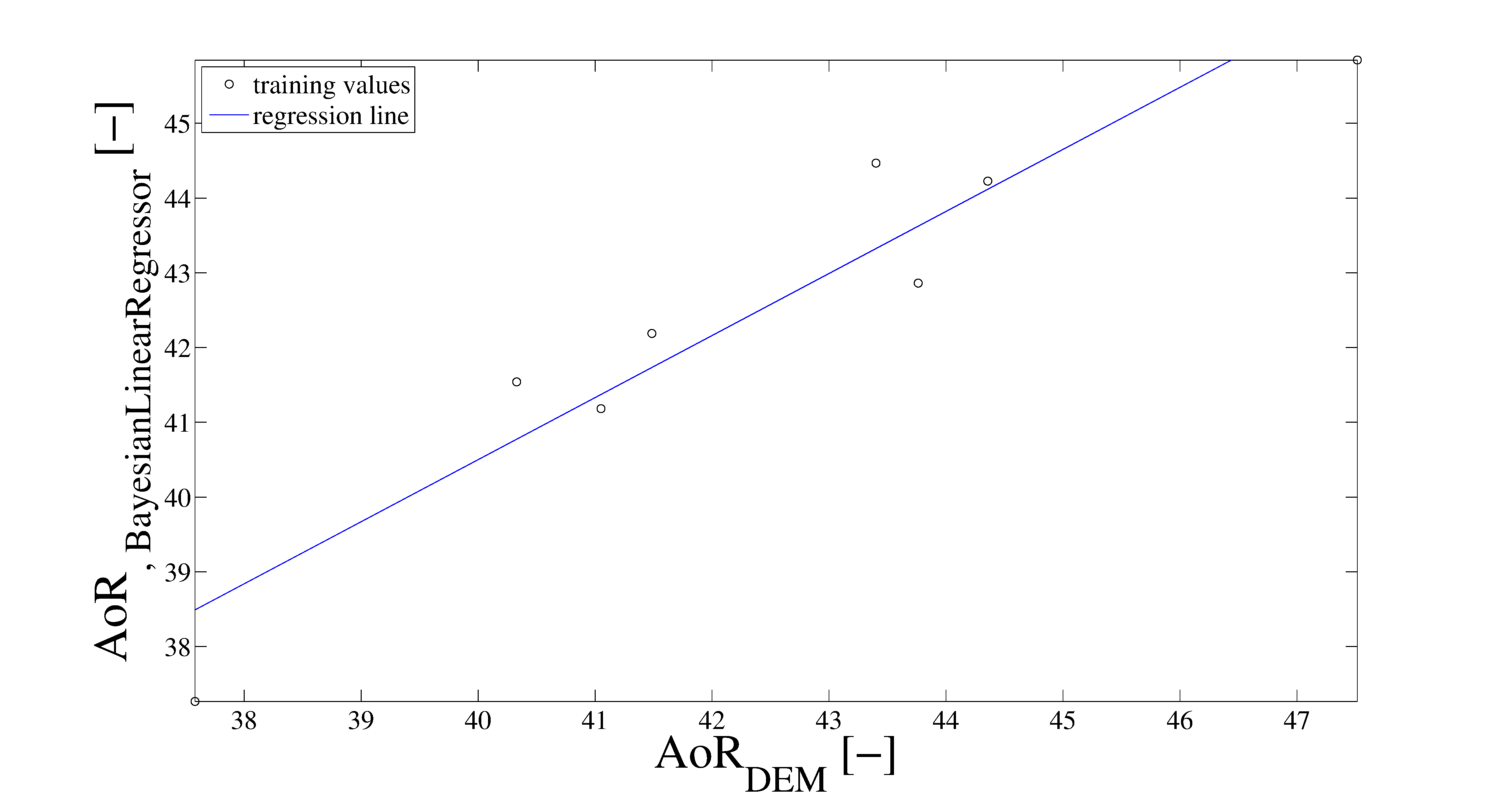
\includegraphics[width=.75\columnwidth]{images/140AoRBayesianLinearRegressor}
	  \label{fig:140AoRBayesianLinearRegressor}  }
  \\
    \subfloat[AoR Gaussian non linear regressor.]{
	  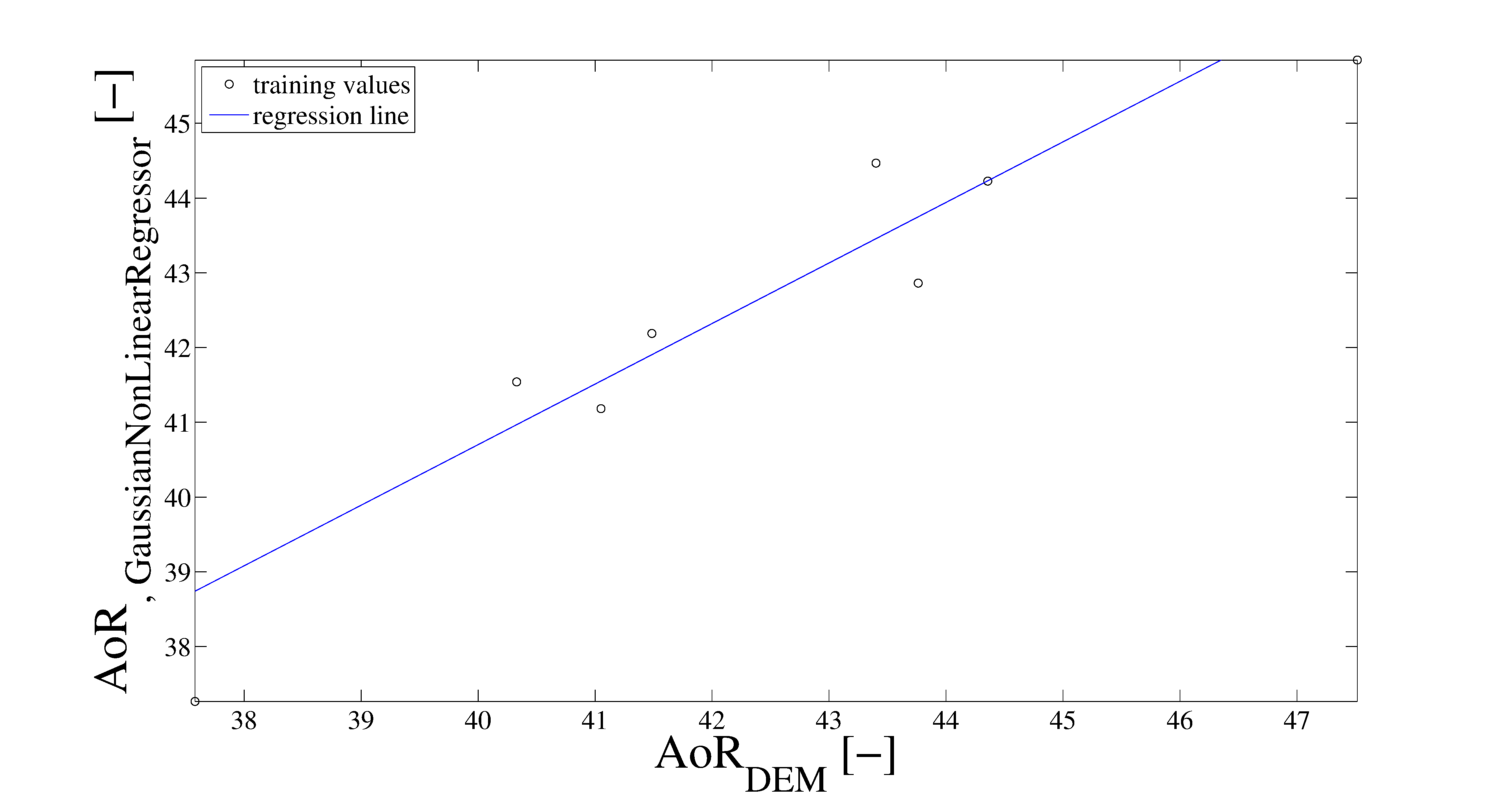
\includegraphics[width=.75\columnwidth]{images/141AoRGaussianNonLinearRegressor}
	  \label{fig:141AoRGaussianNonLinearRegressor}
  }
  \\
 % \hfill
  \subfloat[AoR ANN non linear regression.]{
	  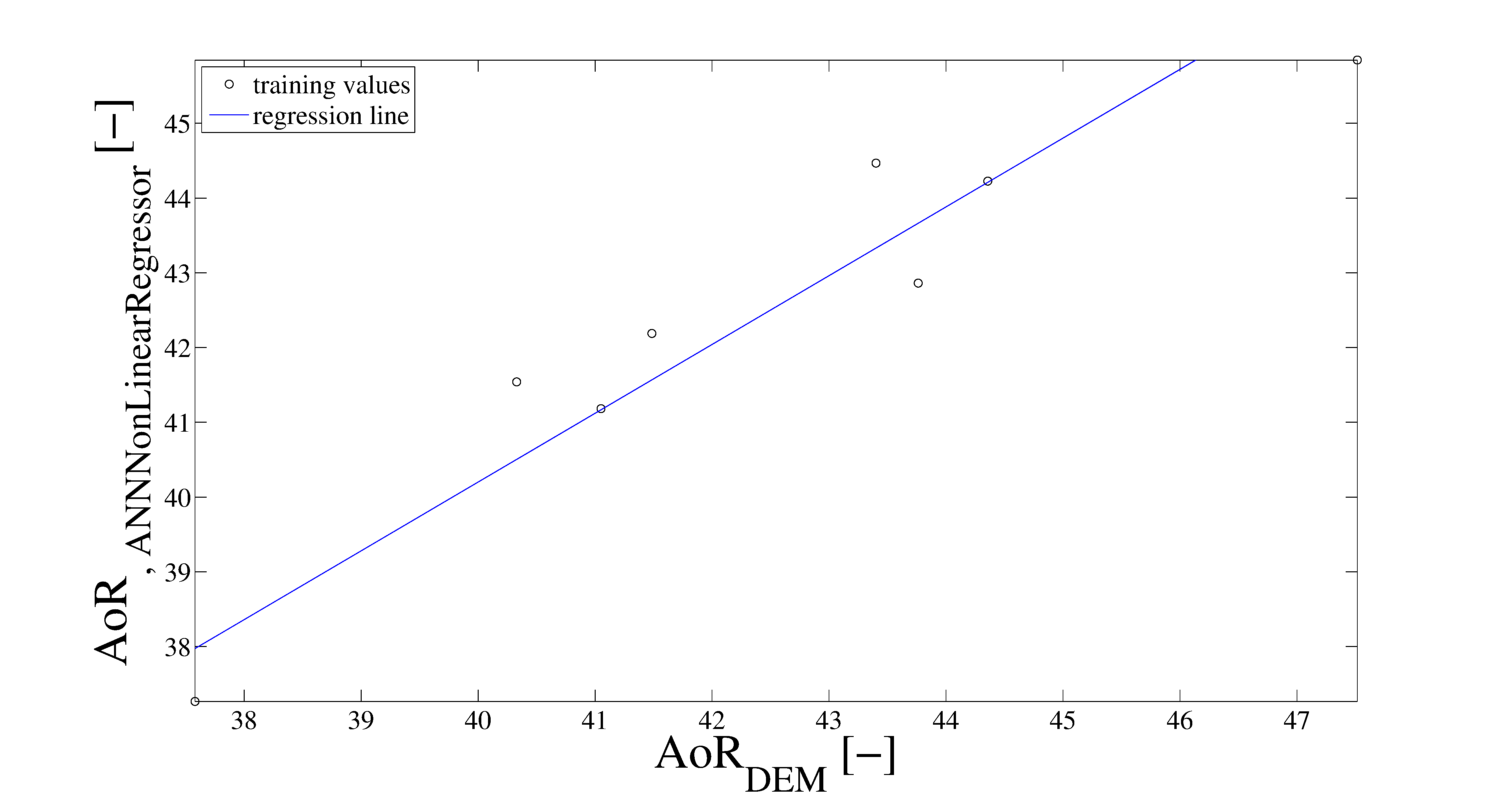
\includegraphics[width=.75\columnwidth]{images/142AoRANNNonLinearRegressor}
	  \label{fig:142AoRANNNonLinearRegressor}
  }
 % \hfill\null
  \caption{Regressions comparison for the \acs{AoR}.}
  \label{fig:144aorregressions}
\end{figure}

% \begin{figure}%[!h] 
% \centering 
% 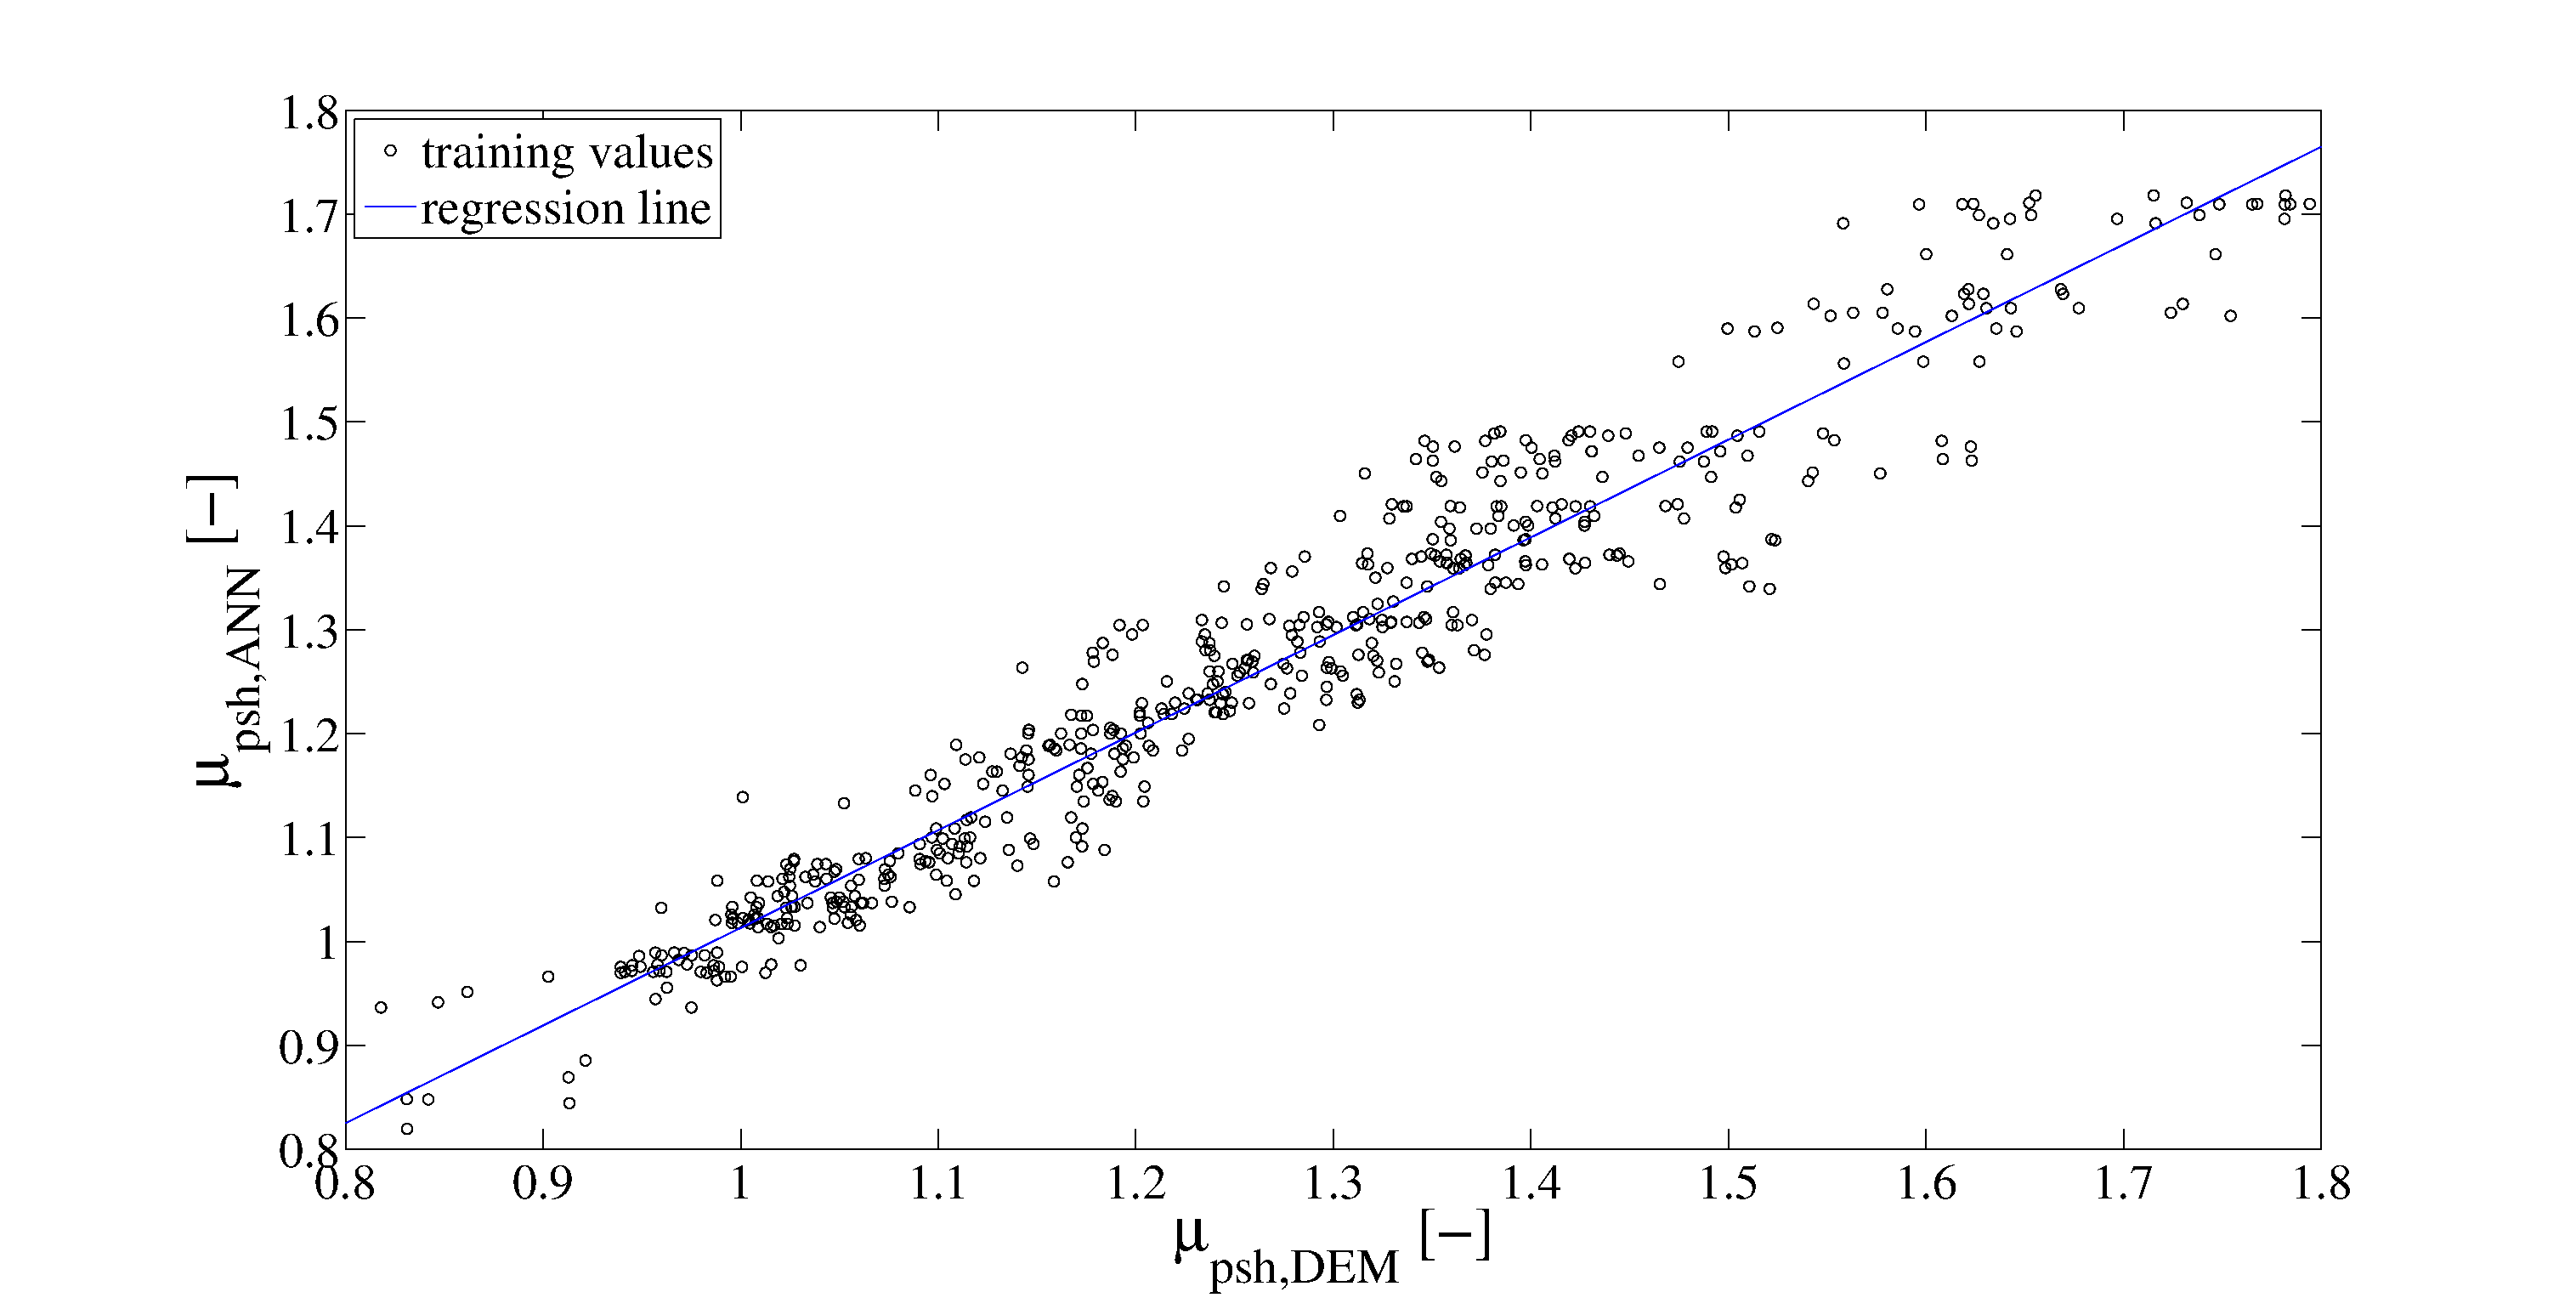
\includegraphics[width=.80\columnwidth]{images/022regression.eps}
% %[width=.48\textwidth]
% \caption[Comparison between prediction of the trained ANN and full DEM
% simulation]{Comparison between prediction of the trained Artificial Neural
% Network (\acs{ANN}) and 546 
% \wrong{write down all the simulations performed at the end.}
% full DEM simulations of the coefficient of pre-shear
% (\acs{mupsh}).}
% \label{fig:022regression} 
% \end{figure}